\section{Research Work and Results: the quantile Framework}

In this part, we are going to change the goal, and try to maximise a quantile of the distribution, instead of the mean. Indeed, sometimes we may have specific applications where the mean doesn’t matter so much, but where it is very important to have a safe policy, i.e. to have higher quantiles, even at the cost of lower mean. In the same way, it can be interesting to find more risky behavior on some environment, with higher possible reward, but at the cost of failing more often.\\

Quantile Optimization is a topic well studied in finance, in the framework of portfolios. However very few tackled this issue in the case of MDP. In their paper \cite[Morimura et al.]{morimura_parametric_2012} try to apply their first distributional approach on an Q-learning algorithm trying to optimise quantiles. Even though they obtained empirically promising results, no theoretical results have been obtained se far. A main reason for that is because quantiles are particularly hard to compute. Fearless, we will still try to tackle this topic.\\

First it is important to notice that, as the goal changed, many assumptions that were made in the original case are to be studied again in this case. The theory as to be redone from 0.

\subsection{Framework}

We are still considering MDPs of the form $\MM(\XX,\AAA, P,R, \gamma)$, but with another value to optimize. We consider $x \in \XX$ a specific state, and $\tau \in [0,1]$ the quantile of interest. Our objective is:

\[\max_\pi V_\tau(x) = q_\tau\left(\sum_{t = 0}^{\infty} \gamma R_t \ |\ X_0 = x\right) \]

Among the result that we are interested in finding back are the Bellman Optimality Principle, the sufficiency of deterministic policies and the computation of the different quantiles. Those are all results and algorithms that used some properties of the mean, mainly its linearity, which we do not have anymore.

\subsubsection*{Policy Evaluation}

The first question, just as before, is how to evaluate a policy. Let $\pi$ a policy. We want to compute:

\[ Q_\tau(x,a) = q_\tau\left(\sum_{t = 0}^{\infty} \gamma R_t \ |\ X_0 = x, A_0 = a, \pi\right) \]

When working with the mean, we would profit of its linearity to find an equation verified by this quantity, and solve this equation. Here, there is no linearity. In fact, is not even possible to compute a quantile solely knowing the quantiles for the next statest and action. We require the full distribution of the reward and the full distribution of reward and next state-action return. 

With the development of the distributional approach, we have a way to compute the full distribution of the return for a specific policy. And once the distribution is known, so is the quantile.\\

In the case where it only requires a finite number of (distributional) Bellman operator application to get the exact distribution, we get to compute the quantile exactly. This happens for instance in MDP that ends after a finite number of steps.\\

if

\[\exists k \in \NN,\ \forall \eta_0 \in \PPPP(\RR)^{\XX \times \AAA}, (\TT^\pi)^k\eta_0 = \eta_\pi \] 
then
\[ \forall \eta_0 \in \PPPP(\RR)^{\XX \times \AAA}, q_\tau\left((\TT^\pi)^k\eta_0\right) = q_\tau(\eta_\pi)\]

In the general case, even though we have the convergence of the distribution,it may not be enough for the convergence of the quantile.

\[ (\TT^\pi )^n \eta \underset{n \rightarrow \infty}{\longrightarrow} \eta_\pi \quad \nRightarrow \quad q_\tau\left((\TT^\pi )^n \eta\right) \underset{n \rightarrow \infty}{\longrightarrow} q_\tau(\eta_\pi)  \]

The result on the convergence of the operators tells us that it converges for the Wasserstein Metrics. By definintion of that metric, it means that the quantile function converges for the $L_p$ norm. However we cannot guarantee the point-wise convergence that we would need here. The closest we get is with the Riesz-Fischer theorem, that tells us that we can extract a sub-sequence converging almost everywhere. We can hope that in practice it will work well enough, which it does on the simulations.

Below are exemples of distributions evaluated for the MDP and the policies that will be introduced in the next section. They distribution parametrization was set the categorical one, with a resolution of $500$. The discount parameter was $0.9$. For the convergence, we applied the Bellman Operator $50$ times.

\begin{figure}[!ht]
    \centering
    \begin{subfigure}{0.95\textwidth}
        \centering
            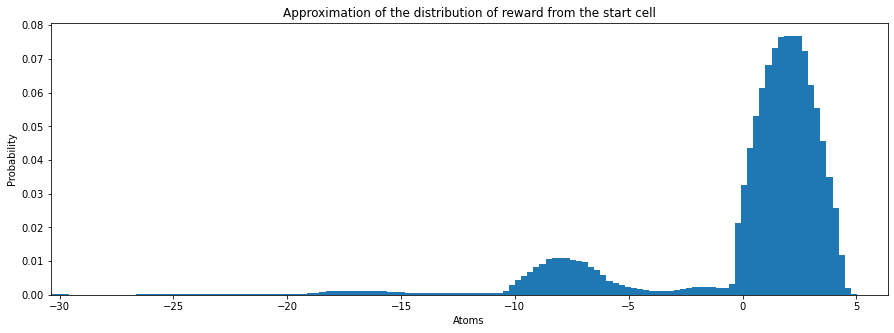
\includegraphics[width=\textwidth]{figures/personal_work/distrib_safe_policy2.png}
        \caption{Safe policy distribution}
        \label{SafeDistrib}
    \end{subfigure}
    \hfill
    \begin{subfigure}{0.95\textwidth}
        \centering
        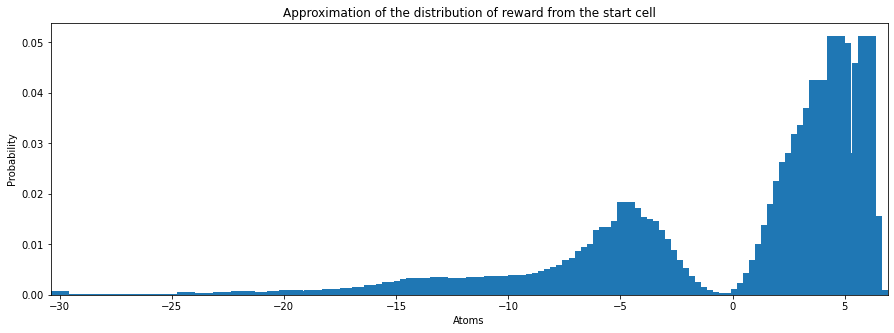
\includegraphics[width=\textwidth]{figures/personal_work/distrib_greedy_policy.png}
        \caption{Risky policy distribution}
        \label{GreedyDistrib}
    \end{subfigure}
        \caption{Examples of return distributions}
\end{figure}

\subsection{Environment of tests}

To try to understand the behavior of this new Framework we had to choose an test environment. We chose to experiment on the Cliff environment, introduced by [Sutton and Barto], which is also the one used in the article of [Morimura et al.].

\begin{figure}[!ht]
    \centering
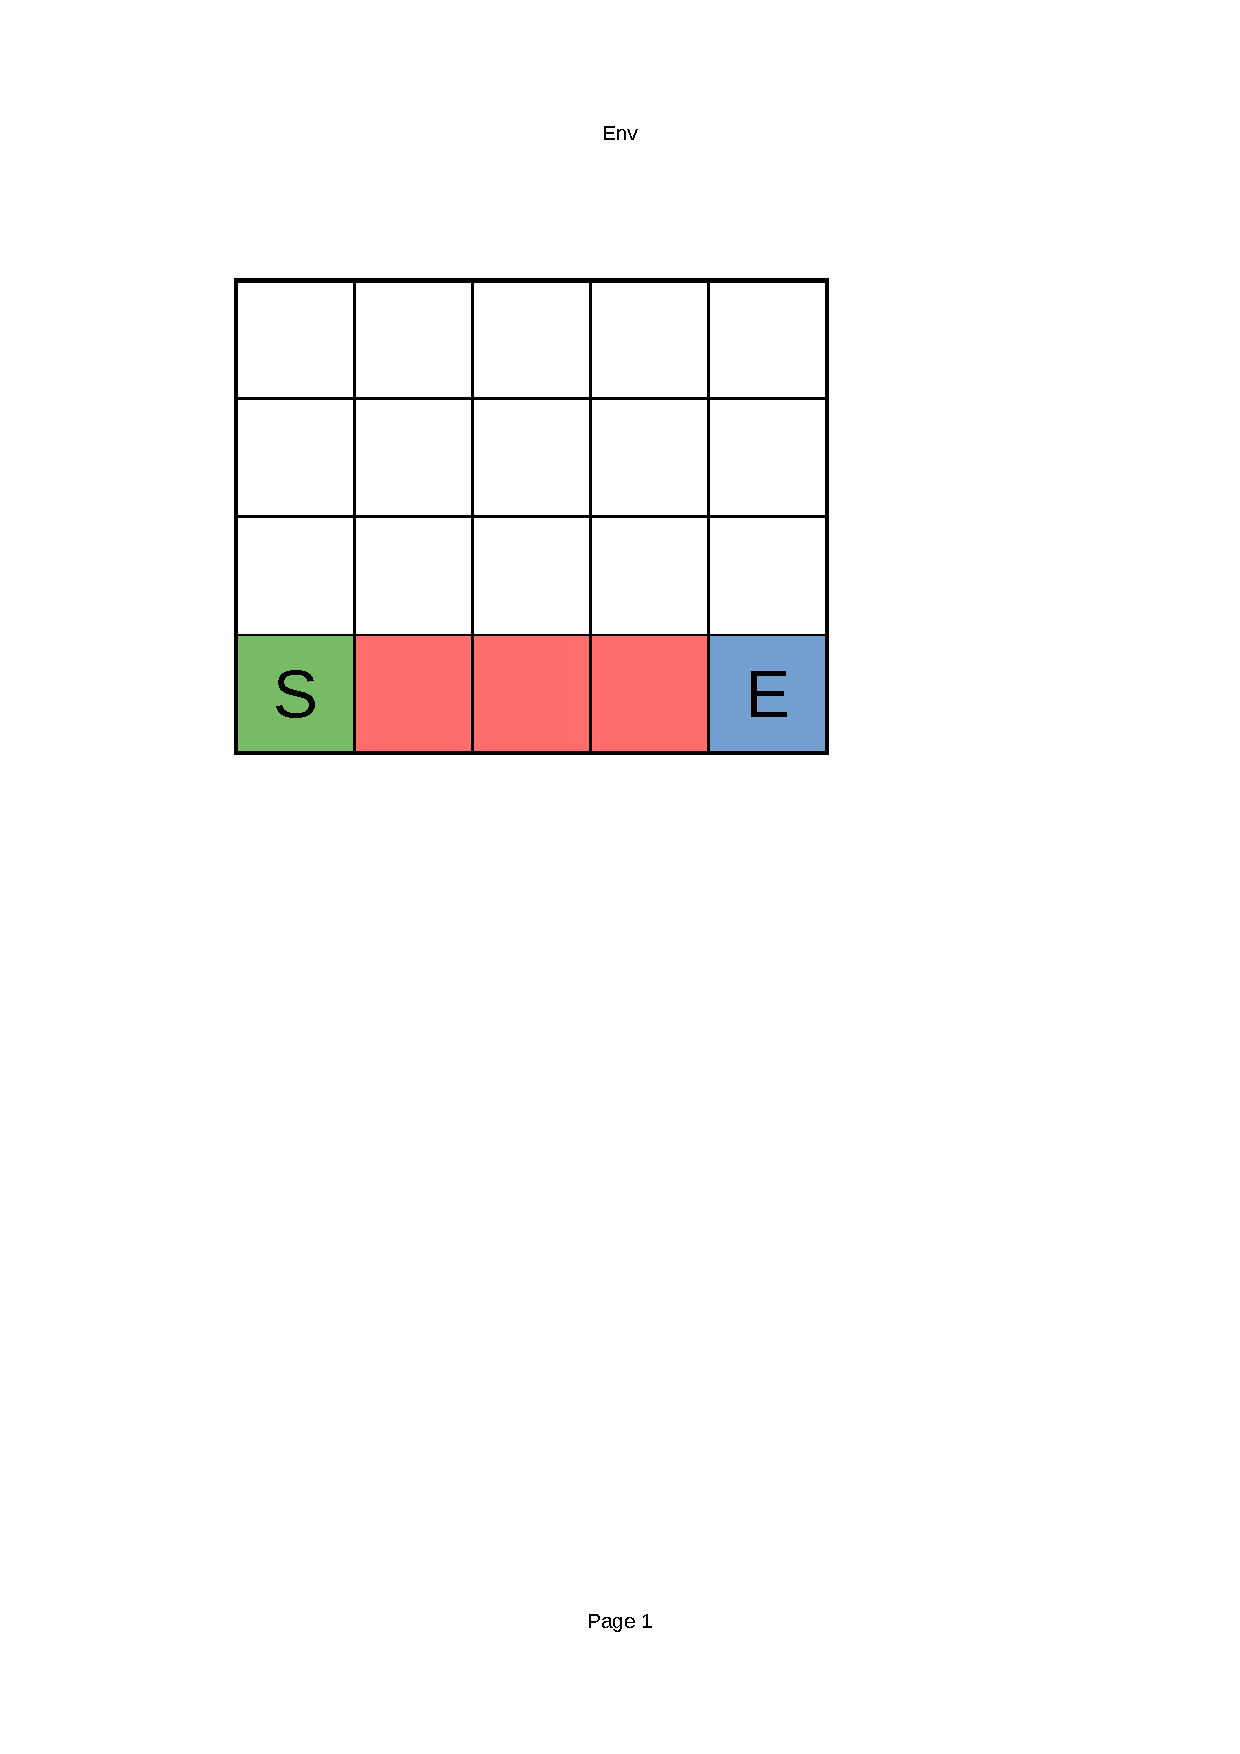
\includegraphics[page=1, trim = 40mm 160mm 70mm 45mm, clip, height=0.2\textheight]{figures/personal_work/policies.pdf}
\caption{State space of the Cliff environment}
\end{figure}

This environement is represented by a grid with a starting state (S), and a terminal state (E). There is also a pit between the two. The goal of the agent is to go from S to E without falling. The reward received when reaching E is set to $10$. The reward received when falling is set to $-10$ and when the agent does, it is teleported back to the start and has to start again. The agent can move in the $4$ directions. When it hits a wall, it doesn’t move. To add some random in it, at each step the agent has only $0.7\%$ chances to go in the chosen direction, and has $0.1\%$ chances to go any other direction.

This environment is particularly well suited for risk-sensitive RL, as it is easy to define safe and risky policy on it, making it easier to evaluate those new algorithms.

\begin{figure}[!ht]
    \centering
    \begin{subfigure}{0.45\textwidth}
        \centering
            \includegraphics[page=2, trim = 40mm 160mm 70mm 45mm, clip, height=0.2\textheight]{figures/personal_work/policies.pdf}
        \caption{Safe policy}
        \label{SafePolicy}
    \end{subfigure}
    \hfill
    \begin{subfigure}{0.45\textwidth}
        \centering
            \includegraphics[page=3, trim = 40mm 160mm 70mm 45mm, clip, height=0.2\textheight]{figures/personal_work/policies.pdf}
        \caption{Risky policy}
        \label{RiskyPolicy}
    \end{subfigure}
        \caption{Example of policies}
\end{figure}

We chose a fixed set of parameters, and tested policy iteration on it, with different optimization criterion: optimization on the mean, on the median, on the quantile 20, on the quantile 0.8. We chose the quantile projection, with a resolution of 500, we each time applied the Bellman operator 50 times (except for the quantile 0.2), the discount $\gamma$ was set to $0.99$.

The results for the mean, is the following. The algorithm converges, as expected. The optimal policy for the chosen parameters is an in-between of the safely and the safe policy. At first it acts greedily, but reaching the end, the agent find it better to just risk it and trying to get sooner, with higher risks of falling, rather than playing it safe and arriving later with a discounted reward. The importance of the discounted is highlighted when comparing with a lower discount: the agent acts more risky as taking detours decreases much more the rewards.

\begin{figure}[!ht]
    \centering
    \begin{subfigure}{0.25\textwidth}
        \centering
            \includegraphics[page=5, trim = 40mm 160mm 70mm 45mm, clip, width=0.95\textwidth]{figures/personal_work/policies.pdf}
        \caption{Optimal policy}
    \end{subfigure}
    \hfill
    \begin{subfigure}{0.70  \textwidth}
        \centering
            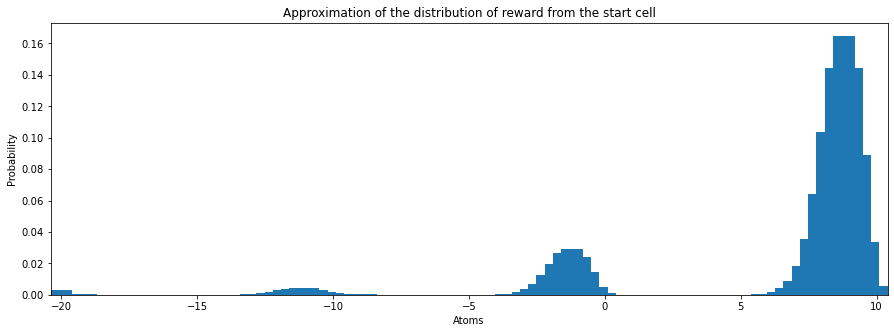
\includegraphics[ width=\textwidth]{figures/personal_work/distrib_mean_99.png}
        \caption{Optimal distribution of return}
    \end{subfigure}
        \caption{Behavior on mean optimization $\gamma = 0.99$}
\end{figure}

\begin{figure}[!ht]
    \centering
    \begin{subfigure}{0.25\textwidth}
        \centering
            \includegraphics[page=4, trim = 40mm 160mm 70mm 45mm, clip, width=0.95\textwidth]{figures/personal_work/policies.pdf}
        \caption{Optimal policy}
    \end{subfigure}
    \hfill
    \begin{subfigure}{0.70\textwidth}
        \centering
            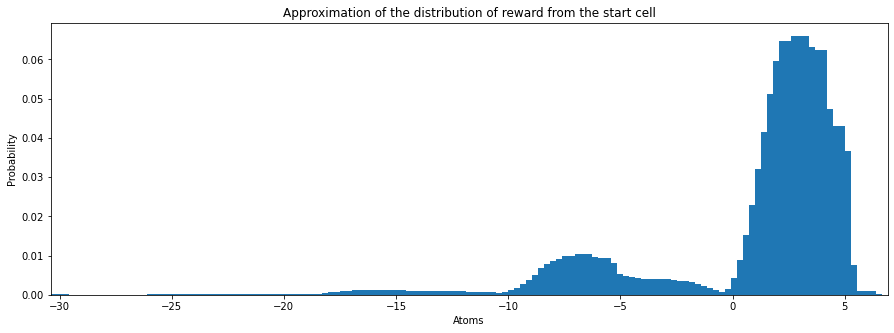
\includegraphics[ width=\textwidth]{figures/personal_work/distrib_mean_9.png}
        \caption{Optimal distribution of return}
    \end{subfigure}
        \caption{Behavior on mean optimization, $\gamma = 0.9$}
\end{figure}

The case with median is more complicated. The algorithm runs but does not converge. It ends up stuck in a loop of period 4. The following policy are what it is stuck with. On the policy we can see that at some cells, the algorithm find it better to go down. It doesn’t seem to make sens since, be it for a quantile or for the mean, it should always be better to go the right first: it gets as close to the end cell, but stay further from the edges. By analysing the value distribution function obtained, it was shown that this behavior was due to the two actions leading to the same quantile, even though going to the right was better mean-wise. In our implementation, in case of equality, the first action with maximum objective would always be chosen, which here was the down direction. In terms of theory, the quantile was equal because of the approximation necessary in the distribution parametrization, but should not be otherwise. Unfortunately, increasing the resolution would not fix the issue. Interestingly enough, this strange behavior would still result in a better median reward than the mean case.


\begin{figure}[!ht]
    \centering
    \begin{subfigure}{0.24\textwidth}
        \centering
            \includegraphics[page=8, trim = 40mm 160mm 70mm 45mm, clip, width=0.95\textwidth]{figures/personal_work/policies.pdf}
        \caption{1st output policy}
    \end{subfigure}
    \begin{subfigure}{0.24\textwidth}
        \centering
            \includegraphics[page=8, trim = 40mm 40mm 70mm 165mm, clip, width=0.95\textwidth]{figures/personal_work/policies.pdf}
        \caption{2nd output policy}
    \end{subfigure}
        \centering
    \begin{subfigure}{0.24\textwidth}
        \centering
            \includegraphics[page=9, trim = 40mm 160mm 70mm 45mm, clip, width=0.95\textwidth]{figures/personal_work/policies.pdf}
        \caption{3rd output policy}
    \end{subfigure}
    \begin{subfigure}{0.24\textwidth}
        \centering
            \includegraphics[page=9, trim = 40mm 40mm 70mm 165mm, clip, width=0.95\textwidth]{figures/personal_work/policies.pdf}
        \caption{4th output policy}
    \end{subfigure}
        \caption{Policies output by median optimisation}
\end{figure}

For the $0.8$ quantile, it converged and also led to a very greedy policy, with a higher $0.8$ quantile than in the mean case. However we still observe the issue with the agent willing to go down instead of right. 

\begin{figure}[!ht]
    \centering
    \begin{subfigure}{0.25\textwidth}
        \centering
            \includegraphics[page=7, trim = 40mm 160mm 70mm 45mm, clip, width=0.95\textwidth]{figures/personal_work/policies.pdf}
        \caption{output policy}
    \end{subfigure}
    \hfill
    \begin{subfigure}{0.70\textwidth}
        \centering
            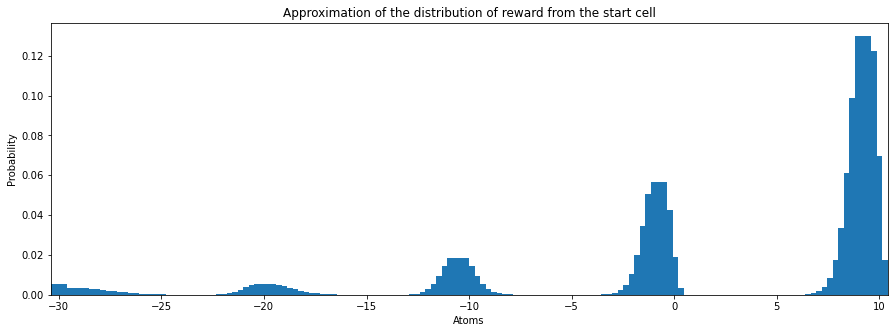
\includegraphics[width=\textwidth]{figures/personal_work/distrib_q80.png}
        \caption{Distribution of return}
    \end{subfigure}
        \caption{Behavior on 0.8 quantile optimazation}
\end{figure}

For the $0.2$ quantile, we observe a much slower convergence, needing twice as many bellman operator applications, but it did converge. We observed a policy quite similar to the one obtained with the mean. However, for this case, the algorithm output a policy that gave a lower $0.2$ quantile than the mean case.

\begin{figure}[!ht]
    \centering
    \begin{subfigure}{0.25\textwidth} 
        \centering
            \includegraphics[page=6, trim = 40mm 160mm 70mm 45mm, clip, width=0.95\textwidth]{figures/personal_work/policies.pdf}
        \caption{output policy}
    \end{subfigure}
    \hfill
    \begin{subfigure}{0.70\textwidth}
        \centering
            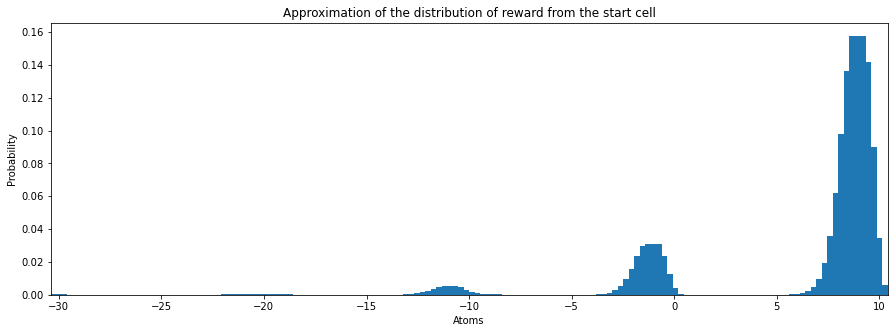
\includegraphics[width=\textwidth]{figures/personal_work/distrib_q20.png}
        \caption{Distribution of return}
    \end{subfigure}
        \caption{Behavior on 0.2 quantile optimization}
\end{figure}
In conclusion, except in a few instances, the algorithms converges and give results quite consistent with what is expected: greedy with a high quantile, safer with a low quantile. However there are cases where it does not converge. The issue seems to be the approximations in the distribution parametrization. Those approximations also lead to specific cases when quantiles are equals for differente action, which can lead to some illogical action choices. Moreover, this issue couldn’t be solved simply by increasing the resolution in the parametrization.

\subsection{Median versus Mean}

When trying to tackle to RL with quantiles, one of our question was to know how does the mean differ to the median. Often in the distribution observed in practice, both are quite close. The previous tests showed that the policy optimizing the mean could differ to the one optimizing the mean, but the median and mean obtained wasn’t significantly different. We wanted how large the difference could to know theoretically. The following example show that the difference in mean can be as high as wanted:

Here a simple example of environment where trying to maximize the median can give an arbitrary difference in mean, compared to the policy maximizing the mean. It also be adjusted to give a significant difference in the median.

\begin{center}
    \begin{tikzpicture} [node distance = 3cm, on grid, auto]
        \node (q1) [state] {$q_1$};
        \node (q2) [state, above left = of q1] {$q_2$};
        \node (q3) [state, above right = of q1] {$q_3$};

        \path [-stealth, thick]
    (q1) edge node {r = 0,M}   (q2)
    (q1) edge node {r = 1}   (q3);
    \end{tikzpicture}
\end{center}

The example consist in an initial state, and two terminal states. There are two actions, one for each terminal states. The first action leads to a reward of $0$ with probability $0.51$, and $M$ with probability $0.49$ ($M$ can be chosen as high as possible). The second action leads to a reward of $1$ with probability $1$. In this MDP, the optimal action for optimizing the median would be the second action, with mean $1$, while the first action would lead to a mean of $M/2$

This example is a great example of the dilemna that is studied when trying to minimize risks: depending on what represents the reward and the context, is it better to have low reward 100\% of the time, is it better to risk not having anything (or worse, having a penalty), but having low chances to get very high reward.

By tweaking the reward and probabilities in this example, it is possible to show that we can obtain any behavior with any quantile. Hence, in the general case, it is not possible to bound the gap between polices maximizing different quantiles and the mean.

\subsection{About dynamic programming}

Even though the approximation issues could have explained why the algorithm wouldn’t work, dynamic programming will not be able to work properly. Indeed, it worked in the general Framework because, with the mean, we had the Bellman Optimality Principle. Unfortunately, this is not the case anymore. The following MDP is a counter-example:

    \begin{center}
        \begin{tikzpicture} [node distance = 3cm, on grid, auto]
            \node (q1) [state] {$q_1$};
            \node (q2) [state, above left = of q1] {$q_2$};
            \node (q3) [state, above right = of q1] {$q_3$};
            \node (q4) [state, above left = of q3] {$q_4$};
            \node (q5) [state, above right = of q3] {$q_5$};

            \path [-stealth, thick]
        (q1) edge node {p = 0.7, r=10}   (q2)
        (q1) edge node {p = 0.3, r=0}   (q3)
        (q3) edge node {2, 3}   (q4)
        (q3) edge node {1, 4}   (q5);    
        \end{tikzpicture}
    \end{center}

On the first state, there is a single action, that have probability $0.7$ to lead to state $q_2$ with reward $10$, and probability $0.3$ to lead to state $q_3$ with no reward. Then on $q3$ There are 2 actions possible, the first one having probabilities $0.15$ and $0.85$ to get reward $2$ and $3$, and the second one, the same probabilities to get rewards $1$ and $4$. We will consider the optimisation on the quantile $0.1$. Optimizing this quantile from state $q_3$ would require to use to go to state $q_4$, with a quantile equal to $2$. However this would lead to a quantile equal to $3$ starting from state $q_1$. Doing the other action leads to a quantile equal to $4$ if starting from state $q_1$. Thus, depending on the state we start from, the actions will be different.\\

This confirms the observation that policy iteration and value iteration algorithms would not work very well in practice. There will be no guarantee that they will work on some instances of choice, and the behavior might be unpredictable. Yet, it doesn’t prevent the algorithms to output policies with better quantiles on some instances, and they could still be worse using.\\

Also, in the mean framework the Bellman Optimality Principle was quite convenient: even when wanting to optimize the return starting to a single beginning state, we would optimize it for every state simultaneously. Here, there is a choice to made, a choice on which state we want the quantile of the return optimized.


\subsection{About policies}
The first result we had on policies in the general framework, was that non-stationnary policies had the same expressive power as stationnary ones and thus, we could restrain ourself the latter. Yet, [Bellemare et al.] show that it was not the case anymore in Distributional RL, and that some distribution could only be obtained through non-stationnary policies.\\
%but what about optimal policies ?

Then, investigating the theoretical properties of the quantile framework was particularly har  because of the quantile itself. Among the few nice properties that it possess, we found this one, which has some implications with how optimal policies behave:

\begin{lemma}
    Let $n \in \NN$, let $0 \leq \lambda_1,\lambda_2,\dots,\lambda_n \leq 1$ such that $\sum_{i = 0}^{n} \lambda_i = 1$, and $\mu_1,\dots, \mu_n $ $n$ distributions. Let $q_\tau$ the quantile function for $\tau \in [0,1]$. We have:

    \[ q_\tau \left( \sum_{i=0}^{n} \lambda_i \mu_i\right) \leq \max_{1 \leq i \leq n} q_\tau ( \mu_i) \]
\end{lemma}
\begin{proof}
    Let $\mu_1,\dots, \mu_n $ probability measures. Let $0 \leq \lambda_1,\lambda_2,\dots,\lambda_n \leq 1$ such that $\sum_{i = 0}^{n} \lambda_i = 1$. Let $\tau \in [0,1]$.
    We denote $q_i = q_\tau (\mu_i)$ and $q_{max} = \max_i q_\tau (\mu_i)$.\\

    Recall that, $\forall \mu$ probability measure, 
    
    \begin{align*}
        q_\tau (\mu) &= \inf \{ x \in \RR : \tau \leq \mu ( ]-\infty, x])\}\\
                     &= \inf \{ x \in \RR :  \mu (  ]x,+\infty[) \leq 1-\tau \}
    \end{align*}

    Hence,
    \begin{align*}
        \forall i, \mu_i \left(]q_{max}, +\infty[\right) \leq \mu_i\left(]q_i, +\infty[\right) \leq 1-\tau
    \end{align*}
    since $q_{max} \leq q_i$ and by monotonicity of the measure.
    Hence,      
    \begin{align*}
        \left( \sum_{i=1}^n \lambda_i \mu_i \right) \left(]q_{max}, +\infty[\right) \leq \sum_{i=1}^n \lambda_i \mu_i \left(]q_i, +\infty[\right) \leq \sum_{i=1}^n \lambda_i (1-\tau) \leq 1-\tau
    \end{align*}
    Therefore, 
    \begin{align*}
        \left( \sum_{i=1}^n \lambda_i \mu_i \right) \left(]q_{max}, +\infty[\right) \leq 1-\tau
    \end{align*}
     which means $q_{max} \geq q_\tau \left( \sum_{i=1}^n \lambda_i \mu_i \right)$
\end{proof}

What this result mean is that, when trying to optimize a quantile, if we have the choice between different distributions and combinations of them, it is always better to only choose the distribution with the highest quantile. This is precisely the situation where are in with the MDP, on one state, we try to choose the policy that will lead to the highest quantile. This suggests that, in value iteration, we can indeed restrain ourselves to an optimal action and not having to look for all convexe combination. This also make us believe in the fact that in any MDP, we should be able to find a deterministic policy that optimizes the quantile of choice.\\

This first result is encouraging, but it is not enough on itself to show that all optimal policies can be chosen to be deterministic. We conjectured it but have only been able to prove it to some restricted MDPs:

\begin{proposition}
    Consider a finite MDP where no state can be visited twice (i.e, without any loops). Consider a state $x \in X$, and $\tau \in [0,1]$. There exist an deterministic policy $\pi^{*}_x$ that optimizes the $\tau$ quantile for state $x$ :
    \[ V_\tau^{\pi^{*}_x(x)} = \max_\pi V_\tau^\pi(x)\]
\end{proposition}
\begin{proof}[Sketch of proof]
    The idea is to write the distribution of reward starting at this state, depending on the distribution of all transition possible and with the coefficient of the policy. This lead to a convexe combination of distribution, where a distribution here would correspond to a \emph{path} in the MDP, and its coefficient would be a multiplication of several policy parameters.

    The previous result tells us that, to optimize the quantile, we can restrain ourself to only one \emph{path}. It coefficient can be set to $1$ and the others to $0$. This leads to all the policy coefficients being either $0$ or $1$, which means we have a deterministic policy.
\end{proof}

\begin{figure}[!ht]
    \centering
    \begin{tikzpicture} [node distance = 2cm, on grid, auto]
        \node (q1) [state] {$q_1$};
        \node (q2) [state, above right = of q1] {$q_2$};
        \node (q3) [state, right = of q1] {$q_3$};
        \node (q4) [state, below right = of q1] {$q_4$};
        \node (q5) [state, right = of q4] {$q_5$};
        \node (q6) [state, above right = of q5] {$q_6$};
        \node (q7) [state, right = of q5] {$q_7$};
        \node (q8) [state, right = of q2] {$q_8$};

        \path [-stealth, thick]
        (q1) edge node {} (q2)
        (q1) edge node {} (q3)
        (q1) edge node {} (q4)
        (q2) edge node {} (q8)
        (q4) edge node {} (q5)
        (q3) edge node {} (q5)
        (q5) edge node {} (q6)
        (q5) edge node {} (q7);    

    \end{tikzpicture}
    \caption{Example of an MDP on which the proposition applies}
\end{figure}

We also tested the conjecture on several simple MDPs that included loops, and everytime it seemed that the optimal policy could be chosen to be deterministic. No counter-example have been found so far. This conforts us in believing in the conjecture. However, the proof has yet to be found. The issue mainly comes from the fact that, with loops, the policies parameters appear several time multiplied to themselves, and the sum is not a convexe combination anymore, preventing us from using our only inequality on quantiles.\\

Having the most general result would be a theoretical advancement in the understanding of the framework, but may not bring much in the practical point of view. Currently, with no dynamic programming, the problem of finding the policy that maximizes a certain quantile is intractable, because of the continuum of possibilites on the policies. Looking only for a deterministic policy would help making the problem exponential in complexity (without considering the approximations necessary when dealing with distributions), which is usually too much for any real application.